\chapter{Grundlagen}
\label{chap:grundlagen}

\section{Begriffserklärungen}
In dieser Arbeit wird ein \emph{Publish/Subscribe-System über einem \ac{p2p} overlay Netzwerk} beschrieben.

\missing{FUFUFU}

\paragraph{Overlay Netzwerk} Ein Overlay-Netzwerk\index{Netzwerk!Overlay} ist ein logischer Aufsatz auf einem bestehenden Netzwerk. Weiterhin zeichnet es sich dadurch aus, dass ein eigener Adressraum genutzt wird und somit das unterliegende Netzwerk überlagert wird. Knoten im Netzwerk können demnach benachbart sein, ohne eine direkte physikalische Verbindung zu haben.\\
Ein Overlay-Netzwerk bietet neben dem eigenen Adressraum auch Funktionalität zum Versand, Empfang und Routing von Nachrichten \cite{Tannenbaum2003}. 

\paragraph{\ac{p2p}-Netzwerk} p2p-Netzwerke\index{Netzwerk!p2p} beschreiben den Verbund von Knoten, sogenannten Peers, die miteinander gleichberechtigt kommunizieren können \cite{Steinmetz2005}. p2p-Netzwerke werden meist durch Overlay-Netzwerke realisiert, da Techniken wie beispielsweise IP-Multicast \cite{Deering1990Multicast} nicht weit verbreitet sind und diese vom unterliegenden Netzwerk abstrahieren. Durch deren angebotene Funktionen können viele Arten von p2p-Systemen implementiert werden. Grundlagen dieser Systeme sowie deren unterschiedliche Ansätze werden in \Fref{chap:grundlagen:p2p} näher besprochen.\\
Meist wird unter p2p \emph{Filesharing} verstanden, was aber nicht immer der Fall sein muss. Geeignete p2p-Netzwerke können unter Anderem auch als Kommunikationsnetze genutzt werden \cite{Darlagiannis2006Peertopeer}.

Im Folgenden werden die Begriffe \emph{p2p-Netzwerk} und \emph{Overlay-Netzwerk} in dieser Arbeit synonym benutzt. In vielen zitierten Arbeiten wird von \emph{p2p-overlay network} gesprochen und dies drückt die Anforderung dieser Arbeit an solche Netzwerke aus:\\
Ein vom physischen Netzwerk (räumlich) unabhängiger Verbund aus gleichberechtigten Knoten die miteinander kommunizieren können.

\paragraph{Publish/Subscribe-System} Ein Publish/Subscribe-System\index{Publish/Subscribe} beschreibt ein Abosystem. Ein Subscriber schreibt sich bei einem Publisher ein und wird von diesem über Veränderungen benachrichtigt. Solch ein System kann kanalbasiert oder filterbasiert sein. In \Fref{chap:grundlagen:pubsub} sind diese Systeme weitaus genauer aufgeführt. So werden aktuelle Systeme gegen die Anforderungen dieser Arbeit geprüft und daraus Konzepte für das zu entwickelnde System gezogen.

\missing{MÄH, HÄSSLICH!!}

\missing{Irgendein Zitat (Buch)!}


\section{p2p-Netzwerke}
\label{chap:grundlagen:p2p}

IP-Multicast ist eine Möglichkeit ein verteiltes \ac{p2p}-System aufzubauen \cite{Deering1990Multicast}. \ac{p2p}-Netzwerke setzen meist auf Overlay-Netwerke\index{Netzwerk!Overlay} auf, da IP-Multicast nicht weit verbreitet ist\footnote{Es erfordert spezielle Router und entsprechende Infrastruktur.}. Sie sind ein logischer Aufsatz auf einem bestehenden Netzwerk und abstrahieren von diesem durch einen eigenen Adressraum. Knoten im Netzwerk können benachbart sein ohne eine direkte physikalische Verbindung zu haben. Ein Overlay-Netzwerk bietet neben dem eigenen Adressraum auch Funktionalität zum Versand, Empfang und Routing von Nachrichten \cite{Tannenbaum2003}. Overlay-Netzwerke sind vielschichtiger Natur. So sind z.B. der EMail-Dienst mit seinem eigenen Namensraum, Twitter oder Facebook als Overlay-Netzwerke zu bezeichnen. p2p-Netzwerke\index{Netzwerk!p2p} selbst beschreiben den Verbund von Knoten, sogenannten Peers, die miteinander gleichberechtigt kommunizieren können \cite{Steinmetz2005}. p2p-Netzwerke sind vom unterliegenden physischem Netzwerk unabhängig, da sie auf Overlay-Netzwerke aufbauen. Obwohl Overlay-Netzwerke und \ac{p2p}-Netzwerke verschiedene Netzwerkarten sind, werden diese jedoch häufig in einem Atemzug genannt. In vielen zitierten Arbeiten wird ebenfalls von \emph{p2p overlay network} gesprochen; dies drückt die Anforderung an solch ein Netzwerk aus:\\
Ein p2p Overlay-Netzwerk ist ein vom physischen Netzwerk (räumlich) unabhängiger Verbund aus gleichberechtigten Knoten, die miteinander kommunizieren können.

Die erste Generation dieser Netzwerke wurde häufig zum Austausch von Dateien verwendet und wird daher vielfach mit dem Begriff \emph{Filesharing} assoziiert. p2p-Netzwerke werden jedoch auch als Kommunikationsnetze genutzt \cite{Darlagiannis2006Peertopeer}. Der einfache Netzaufbau, die Fehlertoleranz bei ausfallenden Knoten sowie der Wegfall teurer Server lässt diese Netzwerkart auch für Computerspiele interessant werden \cite{Knutsson2004Peertopeer, Triebel2008Peertopeer}. Roussopoulos stellt in \cite{Roussopoulos20032} einen allgemeinen Entscheidungsbaum für und wider den Einsatz von p2p-Netzwerken zur Verfügung. Auch für Sensornetzwerke ist der Aufbau eines p2p-Netzwerkes von Vorteil \cite{MuneebAliandKoenLangendoen2007Case}. Es können wertvolle Ressourcen (z.B. Batterie) besser genutzt werden \cite{Sioutas2009Building}, da die Kommunikation zwischen den Knoten weniger Sendeleistung benötigt als es eine Verbindungen zu einem -- eventuell weit entfernten -- Hauptrechner benötigen würde. Solche Netzwerke können beispielsweise zur Erkennung von Waldbränden genutzt werden. Sensorknoten werden über dem zu überwachenden Gebiet abgeworfen und sammeln Daten wie Temperatur und Luftfeuchtigkeit. Verbunden in einem großen p2p-Netzwerk werden die Daten untereinander ausgetauscht. Zur dezentralen Verwaltung und Abfrage genügt es an einem Sensorknoten die Daten abzufragen.

p2p-Netzwerke lassen sich grundsätzlich als \emph{unstrukturiert} oder \emph{strukturiert} klassifizieren \cite{Steinmetz2005, Lua2005Survey} und in Generationen einteilen \cite{Bo2003PeertoPeer}:
\begin{itemize*}
	\item \emph{1G} unstrukturierte Netzwerke
	\item \emph{2G} strukturierte Netzwerke
	\item \emph{3G} strukturierte Netzwerke mit Fokus auf Anonymität, Authentifizierung, Schutz vor Zensur und verschiedenen Rollen der einzelnen Knoten
\end{itemize*}

\subsection{Unstrukturierte Netzwerke}
Unstrukturierte Netzwerke\index{Netzwerk!Overlay!unstrukturiert} zeichnen sich dadurch aus, dass alle Informationen und Dateien durch Suchalgorithmen gefunden werden müssen \cite{Lv2002}. \\
Ein Client tritt dem Netzwerk bei und stellt seine Suchanfrage in das Netz. Werden entsprechende Peers gefunden die diese Suchanfrage beantworten können, werden zum Transfer Direktverbindungen aufgebaut. Aufgrund der einfachen (meist textbasierten) Struktur der Suchanfragen können diese einen großen Wertebereich abdecken.

Im Wesentlichen lassen sich unstrukturierte Netzwerke in die Typen \emph{zentralisiert} und \emph{dezentralisiert} einteilen.

\paragraph{zentralisiert} Knoten im Netz melden eine Liste der verfügbaren Dateien an bekannte Hauptrechner. Suchanfragen werden ebenfalls an diese Rechner gerichtet. Der Suchende erhält eine Liste von potentiellen Peers, die Dateien seiner Suchanfrage entsprechend anbieten. Diese Dateien werden über direkte Verbindungen zwischen den Peers übertragen. Die einzelnen Hauptrechner stellen bei dieser Art von System einen \emph{single point of failure} dar \cite{Eberspaecher2005}.

\paragraph{dezentralisiert} In dezentralen Netzen gibt es keine bekannten Hauptrechner. Damit sich ein neuer Knoten in das Netz einklinken kann, muss diesem mindestens ein bestehender Knoten im Netzwerk bekannt sein. Über diesen Peer tauscht der neue Knoten Informationen aus und baut eine Nachbarschaft auf. Damit Dateien gefunden werden können, wird die Suchanfrage an alle Nachbarn geschickt, sprich die Suchanfrage wird durch das Netzwerk geflutet. Diese senden sie weiter an ihre Nachbarn.\\
Die Suchanfrage kann z.B. mit einer Anzahl an Hops oder einer TTL\footnote{Time to live} in ihrer Reichweite eingegrenzt werden. Potentielle Zyklen müssen bei dieser Art von Suche aufgelöst werden \cite{Lv2002}. Sind Peers gefunden, wird ebenfalls eine direkte Verbindung zur Datenübertragung aufgebaut. 

Beispiele für solche Netzwerke sind Napster (zentralisiert), Gnutella oder BitTorrent (dezentralisiert).

\subsection{Strukturierte Netzwerke}
Strukturierte Netzwerke\index{Netzwerk!Overlay!strukturiert} der zweiten Generation sind oft dezentraler Natur. Ein Datensatz muss nicht gesucht werden, da anhand der Struktur des Netzes die zuständigen Knoten berechnet werden können. Daten können ebenfalls via Direktverbindung übertragen werden, meist wird jedoch das Netzwerk selbst zum Versand genutzt. Hierbei werden die in Nachrichten gepackte Datensätze über verschiedene Peers geroutet. Der dezentralen Art dieser Netze ist geschuldet, dass ein neuer Knoten mindestens einen Peer aus dem Netzwerk kennen muss. Viele Systeme gehen davon aus, dass der neue Knoten aus einer Liste von Peers, den ihm nächst gelegenem Knoten\footnote{Nähe im Sinne von Latenz beziehungsweise räumlicher Nähe} wählen kann und über diesen den Eintritt in das Netz anstößt.

Strukturierte Netzwerke nutzen häufig die Technik der \acf{dht}\footnote{Siehe \Fref{chap:dht} im Anhang}, da diese als Grundlage einer Vielzahl von unterschiedlichen Anwendungen dienen kann \cite{Wehrle2005, Ghodsi2006AlgorithmsDHT}. Grundsätzlich ist jedem Knoten und jedem Datensatz ein Schlüssel aus dem Schlüsselraum des Netzwerkes zugeordnet. Jeder Knoten ist dabei für einen Bereich aus dem Schlüsselraum \emph{zuständig}, dieser Bereich wird netzwerkabhängig ermittelt\footnote{Bespielsweise anhand der numerischen Nähe von Schlüsseln oder der Reihenfolge der Schlüssel.}. Für einen zu Datensatz ist damit der zuständige Knoten bekannt und das zu Grunde liegende Overlay-Netzwerk kann zur Datenübertragung genutzt werden.\\
Hier wird deutlich, dass diese Netzwerke eher der Kommunikation dienen als dem Austausch von Dateien. Darauf aufbauend gibt es unterschiedliche Systeme die sich hinsichtlich Organisation, Routing, Ein- und Austritt von Knoten und dem Verhalten im Fehlerfall unterscheiden \cite{Goetz2005, Lua2005Survey}. Beispiele für solche Netzwerke sind Chord \cite{Hosseini2007Survey}, Pastry \cite{Rowstron2001}, Tapestry \cite{Zhao2001Tapestry,Zhao2004Tapestry} oder CAN \cite{Ratnasamy2001Scalable}. 

Für \ac{m2etis} sind strukturierte Netzwerke besser geeignet, da sie einerseits als Kommunikationsmedium besser nutzbar sind als unstrukturierte p2p-Systeme bei denen meist ein massenhafter Versand der Nachricht über alle Nachbarn (\enquote{flooding}) genutzt wird. Dies widerspricht klar einer optimerten Eventverteilung im gesamten System. Weiterhin lassen sich Datensätze und Zuständigkeiten in strukturierten p2p-Netzwerken einfach berechnen, was auch die Entwicklung der Publish/Subscribe-Komponente begünstigt. Netzwerke der dritten Generation, wie zum Beispiel GNUnet \cite{Bennett2002GNet}, werden in dieser Arbeit nicht näher betrachtet. Die zusätzlich angebotene Funktionalität wird nicht benötigt und würde ob ihrer Komplexität das zu entwickelnde System aufblähen. Daher werden Chord, Pastry und CAN in \Fref[plain]{chap:evaluation_p2p}, das sich der Auswahl eines geeigneten p2p-Netzwerkes zur Verwendung mit \ac{m2etis} widmet, beschrieben und miteinander verglichen.




\section{Verteilte Publish/Subscribe-Systeme}
\label{chap:grundlagen:pubsub}
Konzeptionell lassen sich Publish/Subscribe-Systeme als eventbasierte Systeme betrachten. Auf Grund ihres Aufbaus und der Skalierung  in orthogonalen Dimensionen\index{Publish/Subscribe!orthogonale Dimensionen} \enquote{Raum}, \enquote{Zeit} sowie \enquote{Synchronisation} eignen sich diese gut zur Verteilung von Events in dezentralen Umgebungen \cite{PatrickTh2003Many, Cugola2002Using}.

\begin{figure}[htbp]
\centering

\includegraphics{grafics/pubsub_black_box.pdf}
\caption{Schema eines Publish/Subscribe-Systems}
\label{fig:pubsub_black_box}
\end{figure}

Publisher und Subscriber werden durch das Event-System voneinander getrennt, wie es in \Fref{fig:pubsub_black_box} dargestellt ist.  Publisher und Subscriber sind räumlich voneinander getrennt. Ein Publisher übergibt die Nachricht an das System und hält weder direkte Verbindung mit den Subscribern noch muss der Publisher alle Subscriber kennen. Diese Trennung bezieht sich nicht nur auf verschiedene Komponenten einer Applikation, sondern kann auch über Applikations- oder gar Rechnergrenzen gehen. Die Zeitliche Trennung beschreibt, dass sich ein Subscriber am System anmelden kann obwohl kein Publisher vorhanden ist, analog können Nachrichten publiziert werden ohne dass Empfänger eingeschrieben sind. Je nach Implementierung können Nachrichten zwischengespeichert werden um diese neuen Subscribern zu zustellen. Bei einem Fernaufrufsystem wie \emph{remote proceduce call (RPC)} \cite{Birrell1984Implementing} ist dies nicht möglich, da die Gegenseite existieren muss. Das Senden einer Nachricht ist für den Publisher nicht blockierend und Subscriber warten zudem nicht aktiv auf neue Nachrichten, sondern werden meist per Callback über neue Nachrichten informiert. Damit wird die Verarbeitung vom Event-System aus nebenläufig getriggert.

Diese Arbeit beschäftigt sich ausschließlich mit dezentralen Publish/Subscribe-Sys\-temen, denn \ac{m2etis} zielt darauf ab, die Rechner der Nutzer in einem p2p-Netzwerk zu verbinden und darauf aufbauend die Events zu verteilen. Viele der Grundlagen in diesem Kapitel gelten sowohl für klassische zentrale als auch dezentrale Publish/Subscribe-Systeme, allerdings müssen im verteilten Fall die Verwaltungsinformationen ebenfalls dezentral auf allen Knoten gespeichert, beziehungsweise geeignete Verteilungsalgorithmen gefunden werden. Somit relativiert sich die Dimension der räumlichen Trennung, da Publisher wie Subscriber Teil des Eventsystems sind.

Banerjee vergleicht verschiedene Arten zum Aufbau solch eines Multicast-Systemes. \enquote{mesh-first} beschreibt den expliziten Aufbau des Netzwerkes. Die Peers untereinander verändern ihre Verbindungen aufgrund bestimmter Metriken und können auch Netzwerkpartitionen beheben sind somit selbst für das Netzwerk zuständig. Der \enquote{implizte} Ansatz beschreibt Publish/Subscribe-Systeme, die auf einem Overlaynetzwerk aufsetzen und dessen Routingalgorithmus indirekt die Verteilungsstruktur bestimmt \cite{Banerjee2001Comparative}. Ein Beispiel hierfür ist Scribe, das in \Fref{chap:related:scribe} beschrieben wird.

Fiege befasst sich näher mit dem Aspekt der Sicherheit und des Vertrauens zwischen Sender, Empfänger und dem Verteilungsystem \cite{FiegeSecurity}. Behnel stellt verschiedene Aspekte von \enquote{Quality of Service} auf verschiedenen Ebenen eines Publish/Sub\-scribe-Systems vor. Beispielsweise \enquote{Latenz}, \enquote{Bandbreite}, \enquote{Zustellgarantien} für Nachrichten auf Netzwerkebene oder \enquote{Reihenfolge}, \enquote{Validität} oder \enquote{Authentifizierung} von Nachrichten auf Verteilungsebene. Er beschreibt das Verhalten einiger Publish/Subscribe-Systeme hinsichtlich der beschriebenen Aspekte \cite{BeFiMu2006PubSubQoS}. 

Grundsätzlich lassen sich Publish/Subscribe-Systeme in zwei Varianten einteilen: \emph{kanalbasiert}\index{Publish/Subscribe!kanalbasiert} und \emph{filterbasiert}\index{Publish/Subscribe!filterbasiert} \cite{Liu2003Survey}. In kanalbasierten Systemen werden die Nachrichten einzelnen Kategorien zugeordnet. Subscriber können sich für Nachrichten dieser Kategorien anmelden und bekommen diese zugestellt. Filterbasierte Systeme haben diese Einteilung nicht, stattdessen sind Nachrichten typisiert (zum Beispiel nur einfache Datentypen und Zeichenketten) und mit einem Wertebereich versehen. Bei der Anmeldung kann ein Prädikat zur Filterung angegeben werden. Der Knoten empfängt nun nur gefilterte, auf das Prädikat passende Nachrichten.

Verbindet man die Filterung von Nachrichten mit einem kanalbasierten Ansatz gelangt man zu einem \emph{hybriden} System\index{Publish/Subscribe!hybrid}: Einer Anmeldung an einem Kanal kann ein Prädikat übergeben werden. Beispielsweise wird eine Anmeldung am Kanal für Bewegungsnachrichten über ein Gebiet eingeschränkt. Die dezentrale Filterung ist jedoch nur möglich, wenn die Nutzdaten vom System lesbar oder mit filterbaren Metainformationen angereichert sind. Zudem müssen die Prädikate im logisch aufgebauten Verteilungssystem bekanntgemacht werden, damit Nachrichten frühzeitig bei der Verteilung gefiltert werden können. Beispielsweise kann der Eventtyp \emph{Gildennachricht}\footnote{vergleiche \Fref[plain]{chap:grundlagen:szenario}} auf einem filterbaren Kanal abgebildet werden. Als Prädikat kann die Gildenzugehörigkeit des Avatars oder eine Liste der Gildenmitglieder, von denen Nachrichten erwünscht sind, angeben werden.\\
Das von \ac{m2etis} zur Verfügung gestellte kanalbasierte Publish/Subscribe-System kann pro Kanal mit einer eigenen Filterungskomponente versehen werden und somit als hybrides System genutzt werden; dies wird in \Fref{chap:konzeption_pubsub} beschrieben.

Ein prominenter Vertreter verteilter, kanalbasierter Systeme ist Scribe, dessen Funktionsweise im nächsten Abschnitt beschrieben wird.

\subsection[Umsetzung eines kanalbasieren Systemes]{Umsetzung eines kanalbasieren Systemes am Beispiel von Scribe}
\label{chap:related:scribe}
Eine Umsetzung von Publish/Subscribe-Systemen in verteilen Systemen, ist der Aufbau eines Multicast-Trees\index{Multicast-Tree}, d.h. eines durch die Knoten im Netz gebildeten Baumes in dem die Nachrichten verteilt werden. Hierbei wird pro Kanal ein eigener Multicast-Tree aufgebaut. Am Algorithmus von Scribe \cite{Castro2002Scribe}wird diese Struktur beschrieben.

Scribe basiert auf dem strukturierten Overlay-Netzwerk Pastry \cite{Rowstron2001} und erzeugt einen vom Subscriber zum Publischer aufgebauten Baum \emph{reverse path forwarding tree} \cite{Dalal1978}.

\begin{figure}[htbp]
\centering
\resizebox{\textwidth}{!}{%
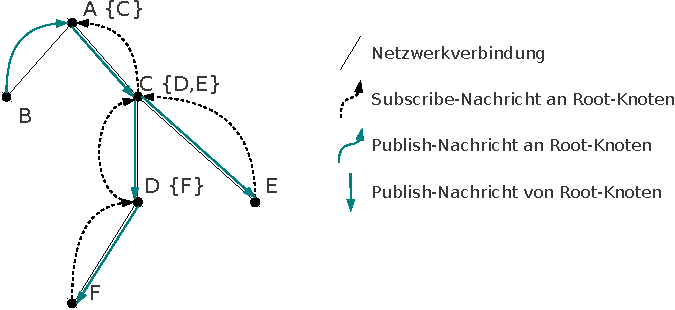
\includegraphics{grafics/multicast_tree.pdf}}
\caption{Schema eines Multicast-Trees}
\label{fig:multicast_tree}
\end{figure}

\Fref{fig:multicast_tree} zeigt ein Netzwerk mit den sechs Knoten A-F. Die Verbindungen der Knoten werden durch dünne schwarze Linien dargestellt. Beispielsweise hat Knoten C Verbindungen zu A, B, D und F.\\
Der Multicast-Tree benötigt einen Knoten, der die Wurzel (im Folgenden \emph{Root-Knoten} genannt) darstellt. Aus Hashwert des Kanalnamens wird ein Schlüssel berechnet. Derjenige Knoten, der aufgrund der Netzwerkmetrik für diesen Schlüssel zuständig ist, wird Root-Knoten des Kanals. Im abgebildeten Falle ist dies Knoten A.\\
Weiterhin hält jeder Knoten eine Liste bei ihm angemeldeter Knoten. In der Abbildung wird diese Liste durch geschweifte Klammern nach der Knotenbezeichnung dargestellt.

\paragraph{Subscribe}
Knoten F sendet eine \emph{subscribe}-Nachricht an A. Diese Nachrichten sind in der Grafik durch gebogene gestrichelte schwarze Verbindungslinien mit Pfeil dargestellt. Das Netzwerk würde diese Nachricht über Knoten D und C an A routen. Knoten D lässt die Nachricht terminieren und trägt F in die Liste der Subscriber ein. Knoten D sendet nun selbst eine subscribe-Nachricht an A. C, über den die Nachricht geroutet wird, terminiert diese, trägt D in die Liste ein und sendet selbst eine subscribe-Nachricht an A. A erhält nun diese Nachricht und trägt C in die Liste ein. Damit sind nun insgesamt drei Nachrichten verschickt worden.\\
Wenn sich Knoten E für den Kanal einschreibt, wird die subscribe-Nachricht an A über den Knoten C geleitet. Dieser terminiert die Nachricht und fügt E der Liste hinzu. Da C selbst angemeldet ist, muss keine weitere Nachricht versendet werden.

Scribe fordert periodische Anmeldungen zur Erhöhung der Fehlertoleranz. Ist ein Knoten ausgefallen, routet das Netzwerk die Nachrichten über andere Knoten. Damit kann der Multicast-Tree wieder aufgebaut werden.

\paragraph{Unsubscribe}
Der Austritt aus einem Kanal erfolgt ähnlich zur Anmeldung. Die Nachricht läuft nur bis zum nächsten Knoten und terminiert dort. Der Knoten entfernt den Sender der Nachricht aus seiner Liste und sendet selbst nur eine \emph{unsubscribe}-Nachricht, wenn die Liste leer ist und er selbst nicht angemeldet ist.

\paragraph{Publish}
In \Fref{fig:multicast_tree} möchte Knoten B eine Nachricht im Kanal publizieren. B sendet darauf eine Nachricht an den Root-Knoten A, da dieser für diesen Kanal zuständig ist (gebogene türkise Linie). Nun sendet A diese Nachricht an alle Knoten in seiner Liste (gerader türkise Linie mit Pfeil). Dies ist in der Abbildung nur Knoten C. Dieser sendet sie weiter an D und E. E gibt diese Nachricht direkt an die Applikation weiter, während D die Nachricht an F schicken muss.


Hierbei ist klar ersichtlich, dass zusätzliche Nachrichten verteilt werden müssen, wenn Knoten F eine Nachricht im Kanal publizieren möchte. Diese Nachricht muss erst von Knoten F zu Knoten A wandern, damit A diese Nachricht wieder über die anderen Knoten zurücksendet. Optimierte Versionen dieses Algorithmus können hier ansetzen und zu publizierende Nachrichten nicht mehr an den Knoten senden, der ihnen diese Nachricht geschickt hat. So würde C die Nachricht nur noch an E weiterleiten.

Bayeux \cite{Zhuang2001} ist ein ähnliches System, jedoch auf Basis des Overlay-Netzwerkes Tapestry \cite{Zhao2004Tapestry}. Tapestry entspricht auch der generischen API, somit stellt dies keinen Unterschied zu Pastry dar. Im Gegensatz zu Scribe, wird bei Bayeux der Multicast-Tree vom Root-Knoten aus aufgebaut. Aufgrund der unterliegenden Routingstruktur des genutzten Overlay-Netzwerkes können sich diese Pfade unterscheiden.


Nach diesem Einblick einer möglichen Umsetzung eines kanalbasierten Publish/Sub\-scribe-Systems gibt der kommende Abschnitt am Beispiel von Mercury eine Vorstellung davon, wie filterbasierte Systeme\index{Publish/Subscribe!filterbasiert} in einem dezentralen Netzwerk implementiert sein können.

\subsection[Umsetzung eines filterbasierten Systemes]{Umsetzung eines filterbasierten Systemes am Beispiel von Mercury}
\label{chap:related:mercury}
Zur besseren Vorstellung einer Umsetzung für filterbasierte Publish/Subscribe-Systeme\index{Publish/Subscribe!filterbasiert} wird im folgenden Kapitel Mercury \cite{Bharambe2004Mercury} vorgestellt. Obwohl \ac{m2etis} ein kanalbasiertes Publish/Subscribe-System darstellt \cite{Fischer2010a}, ist es sinnvoll eine möglich Umsetzung eines filterbasierten Systems zu beschreiben um die grundlegenden Unterschiede der Systeme genauer auszuarbeiten. 

Im System gibt es eine Menge an Attributen, die ihrerseits einen definierten Wertebereich haben. Jedes Attribut wird durch einen eigenen Verbund aus Knoten, den sogenannten \emph{Hub}, bearbeitet. Der Wertebereich ist dabei nicht zwingend symmetrisch auf die Knoten verteilt.

\paragraph{Subscribe}
Eine Subscription $S$ ist ein Tupel aus Filterbedingungen über die Attribute (z.B. $S := (5 < x <= 20; y = 15)$) sowie Kontaktinformationen des Knotens. $S$ wird an einen beliebigen Knoten eines Hubs gesendet, der für das Attribut aus der Filterbedingung mit der größten Selektivität zuständig ist. Im Beispiel ist dies Attribut $y$. Im Hub wird $S$ nun zu dem Knoten weitergereicht, der den Wertebereich der Filterung abdeckt. Dort wird $S$ in einer Liste gespeichert.

\paragraph{Publish}
Eine Publikation $P$ ist ebenfalls ein Tupel mit bestimmten Werten der Attribute (z.B. $P := (x = 10; y = 0)$). $P$ wird an \emph{alle} Hubs gesendet und dort zum zuständigen Knoten weitergereicht. Dieser prüft nun die Liste der gespeicherten Subscriptions gegen die neue Publikation. Stimmen beide überein, so wird $P$ an den eingeschriebenen Knoten weitergeleitet.

Mirinae ist ebenfalls ein filterbasiertes Publish/Subscribe-System, stellt den Wertebereich eines Attributes jedoch als Hyperwürfel dar. Eine automatische Anpassung dieser Aufteilung ermöglicht eine schnelle Anpassung der Routingtabelle und damit einen kurzen Weg für die Nachrichten \cite{Choi2005Mirinae}.


\subsection{VON}
\label{chap:related:von}
\ac{von} ist in seinen Grundzügen stark unterschiedlich zu den bisher vorgestellen Umsetzung. \ac{von} nutzt das \ac{p2p}-Netzwerk nicht nur als Kommumnikationsmedium, sondern nutzt dessen Struktur auch als Verteilungsstruktur es Publish/Subscribe-Systems \cite{Hu2006VON}. VON zielt auf die Verteilungsoptimierung von Events zur Positonsänderun, muss allerdings über Applikationswissen verfügen: Die Position des Spielers. \ac{vast} \cite{Backhaus2007Voronoibased} greift das Konzept von \ac{von} auf und testet eine Implementierung auf OpenSIM \cite{Baumgart2007OverSim}.

\begin{figure}[htbp]
\centering
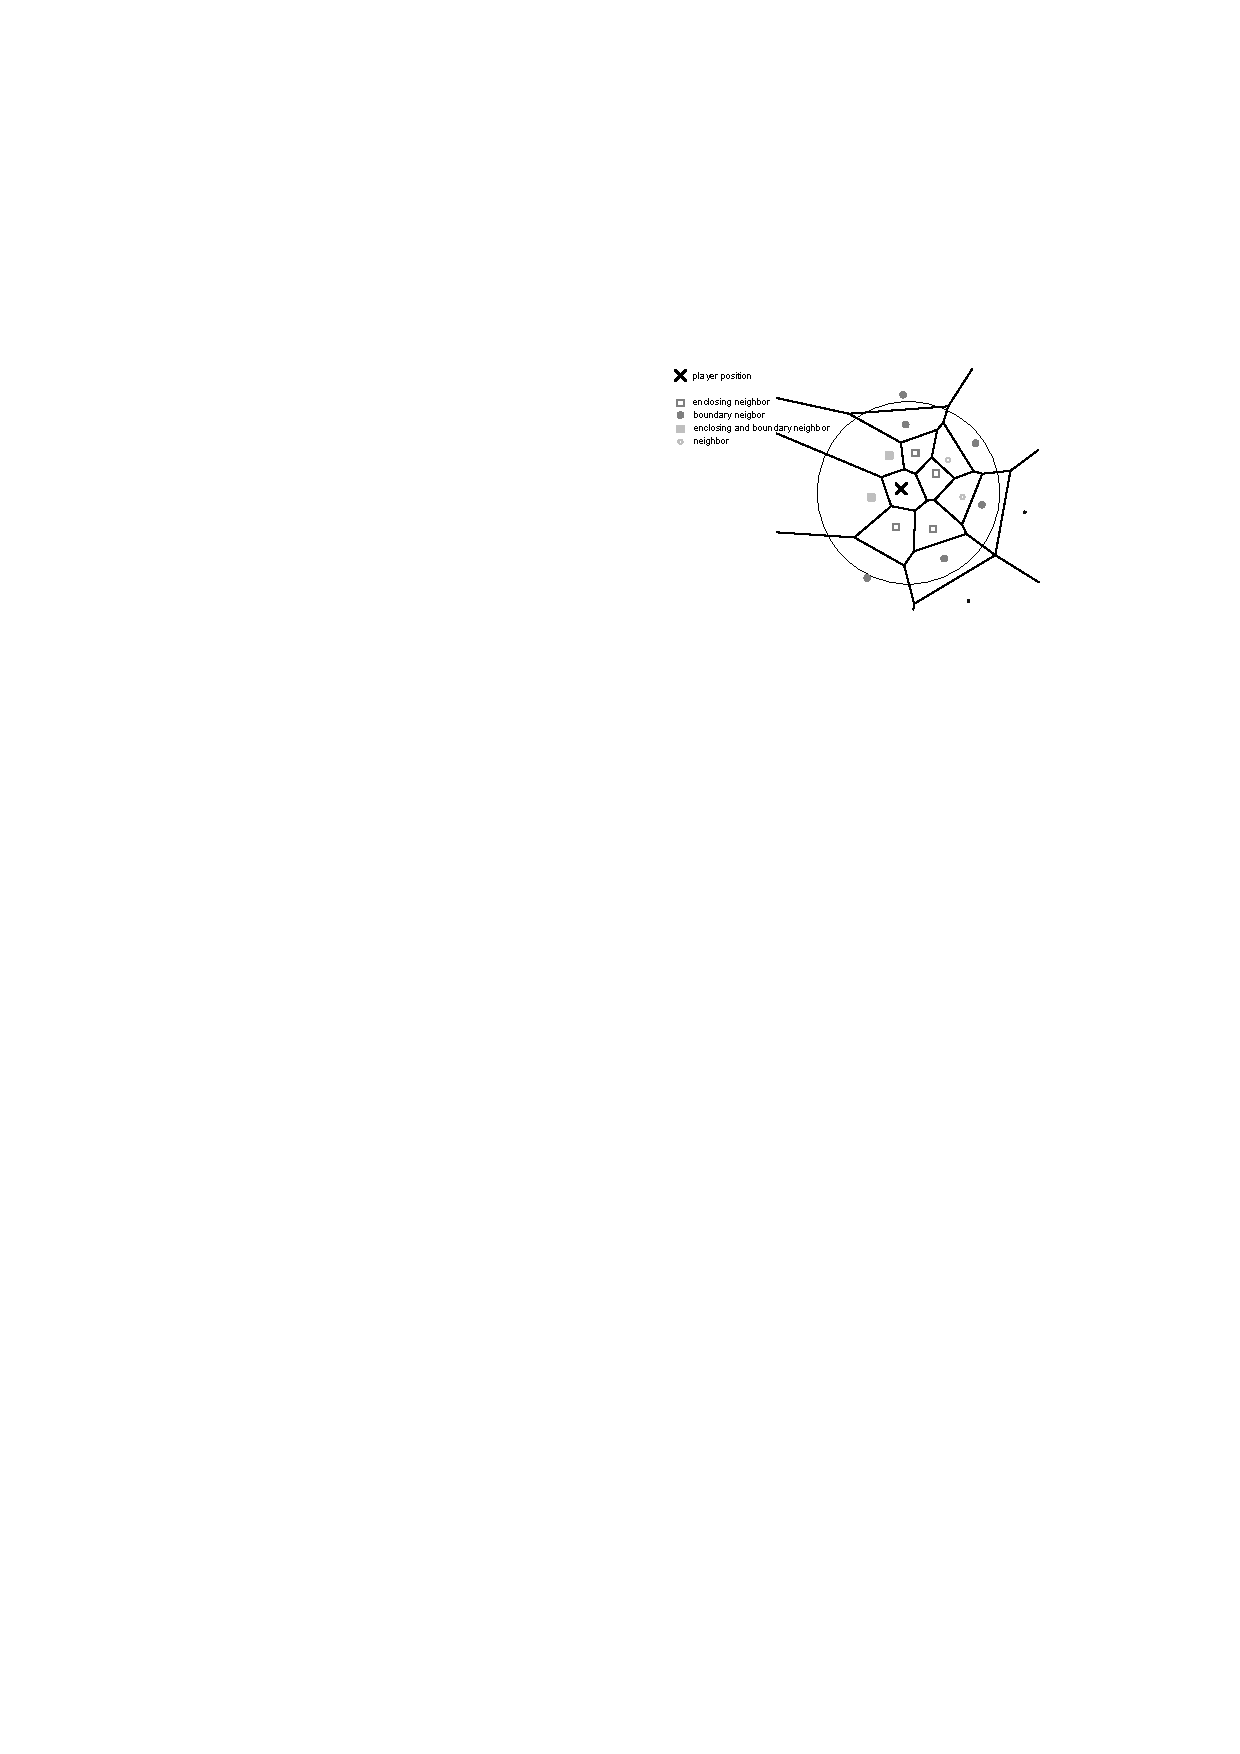
\includegraphics{grafics/voronoi_von_backhaus.pdf}
\caption{Struktur eines VON-Netzwerkes (aus \cite{Backhaus2007Voronoibased})}
\label{fig:von}
\end{figure}

\Fref{fig:von} zeigt einen Aufbau eines VON-Netzwerks. Die Spielwelt wird anhand der Position der einzelnen Knoten in Voronoi-Diagramme unterteilt. Jeder Knoten hat damit einen eigenen Bereich und hält Verbindungen zu seinen Nachbarn und kennt angrenzende Nachbarn im Bereich seiner \ac{aoi}. Anmeldungen im Publish/Subscribe-System sind implizit, denn Publikationen, also Positionsänderungen, werden von einem Knoten an alle direkt angrenzenden Nachbarn (``enclosing neighbor'' in \Fref{fig:von}) gesendet. Um das System konsistent zu halten werden dabei auch Informationen über ``boundary neighbors'' ausgetauscht.


Nach den Grundlagen von \ac{p2p}-Netzwerken, Publish/Subscribe-Systemen und Einblicken in verschiedene Umsetzungen, beschäftigt sich das nächste Kapitel mit der Evaluation dreier \ac{p2p}-Netzwerke m ein geeignetes System als Netzwerk für \ac{m2etis} auswählen.


\section{Betrug}\index{Betrug}
\label{chap:grundlagen:cheating}
Betrug und Betrugsverhinderung bzw. Betrugsvermeidung sind nicht Thema dieser Arbeit. Das zu entwickelnde Framework bietet genug Freiheiten betrugsresistente Publish/Subscribe-Algorithmen einzusetzen oder entsprechende Systeme auf das Framework zu setzen.\\
Dennoch soll dieses Kapitel einen kleinen Überlick über das Thema und die aktuelle Forschung dazu geben.

Betrügerisches Verhalten (Cheating) ist in p2p-Systemen einfacher als in Client/Server-Systemen, da die Kommunikation nicht zwingend über einen (vom Betreiber kontrollierten) Server läuft. Mit gefälschten Nachrichten für Statusmeldungen, wie Positionsänderungen, oder zur Entscheidungsfindung über die Reihenfolge von Aktionen können andere Knoten massiv benachteiligt werden. Das Wissen über das zugrunde liegende System wird genutzt um gezielt wichtige Aspekte des Spieles zu manipulieren.

Webb \cite{Webb2007Cheating} gibt eine Übersicht über Betrug in Netzwerkspielen und geht hier auch auf die Unterschiede zwischen Client/Server-Systemen und p2p-Systemen ein. Cheating wird in vier grundlegende Bereiche eingeteilt: \emph{Game level cheats}, \emph{Application level cheats}, \emph{Protocol level cheats} und \emph{Infrastructure level cheats}. Mögliche Verfahren wie \emph{Lockstep} \cite{Baughman2007}, das die Spielzeit in Runden einteilt, werden vorgestellt und ausgewertet.

\paragraph{Beispiel}
Als Beispiel für einen \emph{Protocol level cheat} wird das Ausnutzen des \emph{Dead-Reckoning}-Verfahrens\index{Dead-Reckoning} \cite{Pantel2002} beschrieben. Dead-Reckoning kaschiert die Latenz im Netzwerk und bietet dem Spieler durch vorberechnete Aktionen der anderen Spieler einen konstanten Spielfluss. Hierbei akzeptiert das System eine gewisse Anzahl an ausgefallenen/verlorenen Updates eines Knotens bevor unterschiedliche Aktionen aus Spielsicht durchgeführt werden.\\
Hält ein Spieler nun eigene Updates zurück, können in der Zeit bis zum geforderten Update die Informationen der anderen Spieler ausgewertet werden. Das Spiel kann somit zu eigenen Gunsten beeinflusst werden. Algorithmen die diese Problematik angehen, werden entwickelt \cite{Aggarwal2005}.

Kabus \cite{Kabus2005Addressing} beschreibt grundsätzliche Techniken die in p2p-Systemen genutzt werden um Betrug aufzudecken beziehungsweise zu verhindern. Beispielsweise können für eine Konsensus\index{Betrug!Konsensus} über Spieleraktionen zufällig Knoten gewählt werden. Diese validieren die Aktionen und können effektiv Betrug verhindern. Natürlich müssen solche Verfahren mit einem erhören Aufwand an Nachrichten teuer erkauft werden.\\
Eine weitere Möglichkeit der Betrugsverhinderung ist das Einsetzen von \emph{trusted hardware}\index{Betrug!trusted hardware} wie es bei Spielkonsolen häufig eingesetzt wird. Hier verhindert die Hardware Spielveränderungen oder den Start von externen Betrugsprogramme, die beispielsweise die Avatarsteuerung übernehmen. Dennoch besitzen auch solche Systeme Schwachstellen und können hintergangen werden.\\
Zur Betrugsaufdeckung führt Kabus die Prüfung von Logdateien an.

Auf weitere zahlreiche Arbeiten zur Betrugsverhinderung beziehungsweise -aufdeckung wird verwiesen \cite{Ferretti2008Cheating, Gauthierdickey2004Low, Kabus2007Design, Dautermann2007, Kabus2009, Castro2002Secure}.


\section{Aufbau von M$^2$etis}
\label{chap:grundlagen:aufbau_metis}

Diese Arbeit entsteht im Rahmen des \ac{m2etis}-Projektes Cite Cite Cite und bla.

Aufbaubildchen

\cite{Fischer2010a, Fischer2010Event}


